\newpage
\section{Fouriersynthese von $f(x)=|sin(x)|$}

Nun lassen sich mit den genannten Formeln die Fourier-Reihe für $f(x)=|sin(x)|$ mit $T=\pi$ folgendermaßen berechnen. Mit \autoref{eq:A_k} lassen sich die Koeffizienten $A_k$ wie folgt berechnen:
\begin{align*}
  A_0 &= \frac{1}{\pi} \int_{-\frac{\pi}{2}}^{\frac{\pi}{2}} | \sin(t) | \symup{d}t \\
  &= \frac{1}{\pi} \int_{-\frac{\pi}{2}}^0 -\sin t \symup{d}t + \frac{1}{\pi} \int_0^{\frac{\pi}{2}} \sin(t) \symup{d}t \\
  &= \frac{2}{\pi} \\
  A_k &= \frac{2}{\pi} \int_{-\frac{\pi}{2}}^{\frac{\pi}{2}} \left| \sin(t) \right| \cos(w_kt) \symup{d}t \\
  &= \frac{2}{\pi} \int_{-\frac{\pi}{2}}^{0} \left( -\sin(t) \right) \cos(w_kt) \symup{d}t + \frac{2}{\pi} \int_{0}^{\frac{\pi}{2}} \sin(t) \cos(w_kt) \symup{d}t \\
  &= - \frac{4}{\pi} \cdot \frac{1}{4k^2-1}
\end{align*}

Und die Koeffizienten $B_k$ wie folgt berechnen:
\begin{align*}
  B_0 &= 0 \\
  B_k &= \frac{2}{\pi} \int_{-\frac{\pi}{2}}^{\frac{\pi}{2}} \left| \sin(t) \right| \sin(w_kt) \symup{d}t \\
  &= \frac{2}{\pi} \int_{-\frac{\pi}{2}}^{0} \left( -\sin(t) \right) \sin(w_kt) \symup{d}t + \frac{2}{\pi} \int_{0}^{\frac{\pi}{2}} \sin(t) \sin(w_kt) \symup{d}t \\
  &= 0
\end{align*}

Damit ergeben sich folgende 18 Koeffizienten für $A_k$

\begin{table}
  \centering
  \caption{Berechnete Koeffizienten für $|\sin(x)|$}
  \label{tab:a_sin}
  \begin{tabular}{c c}
    \toprule 
    $k$ & $A_k$ \\ 
    \midrule 
    0 & 0.6366 \\
    1 & -0.4244 \\
    2 & -0.0849 \\
    3 & -0.0364 \\
    4 & -0.0202 \\
    5 & -0.0129 \\
    6 & -0.0089 \\
    7 & -0.0065 \\
    8 & -0.0050 \\
    9 & -0.0039 \\
    10 & -0.0032 \\
    11 & -0.0026 \\
    12 & -0.0022 \\
    13 & -0.0019 \\
    14 & -0.0016 \\
    15 & -0.0014 \\
    16 & -0.0012 \\
    17 & -0.0011 \\ 
    \bottomrule
  \end{tabular}
\end{table}

\begin{figure}
  \centering
  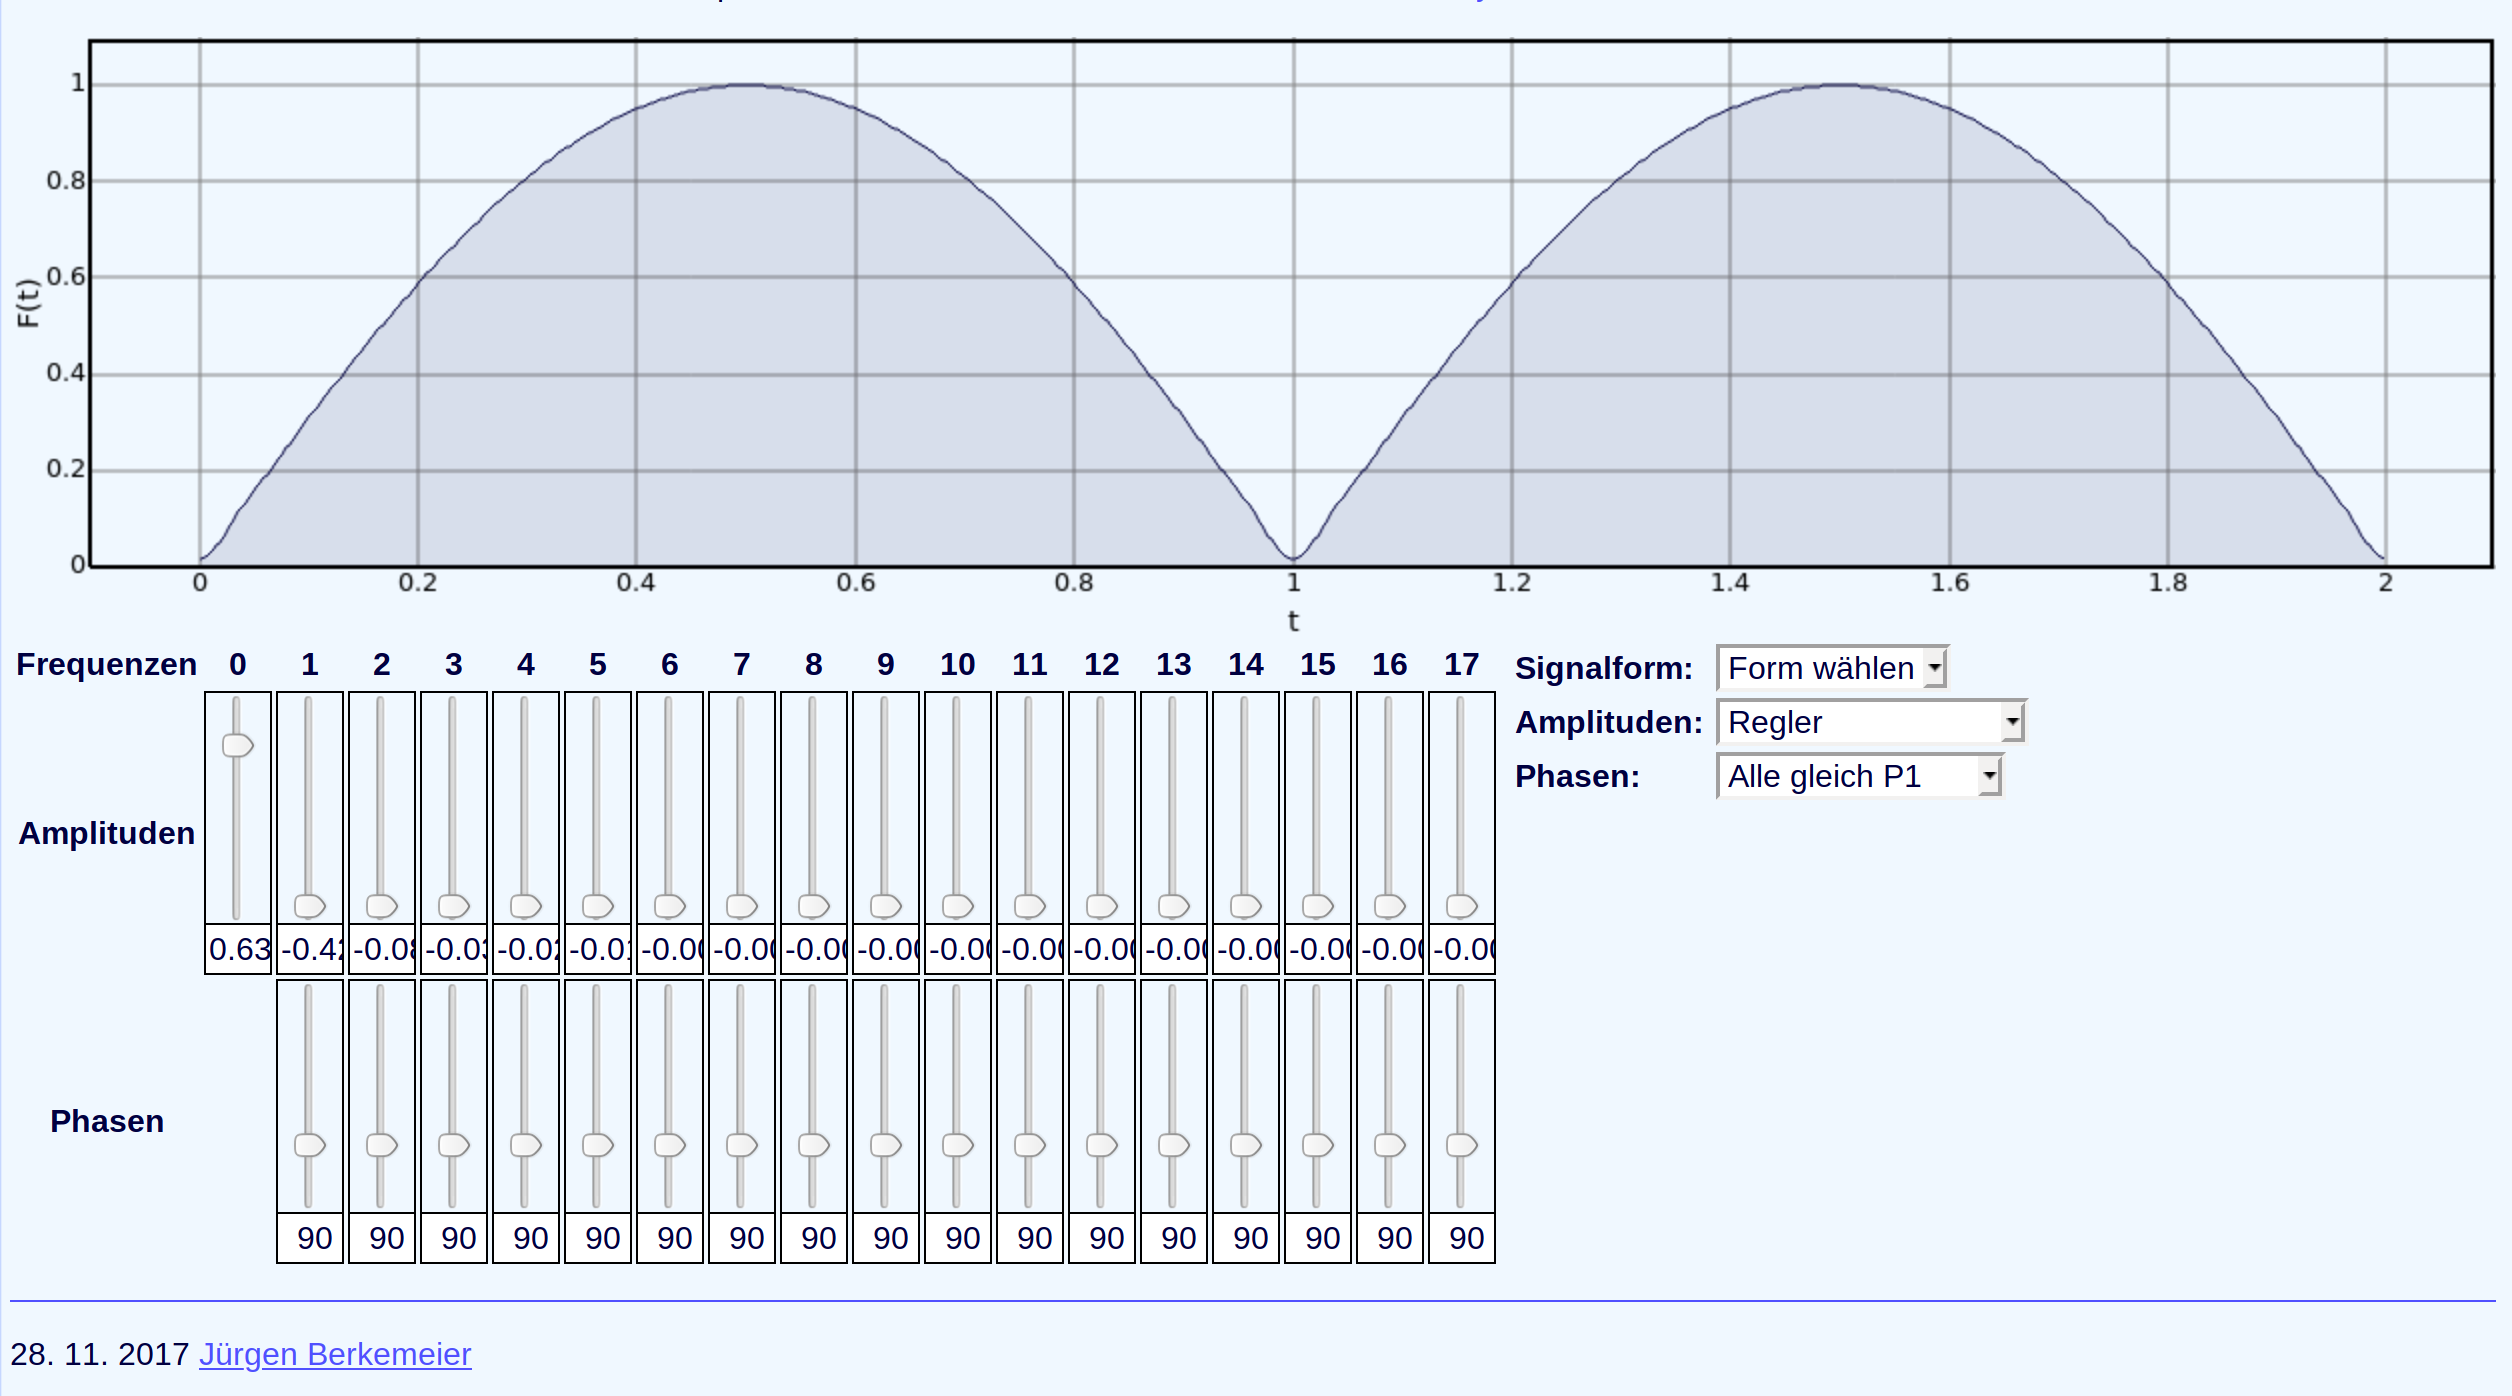
\includegraphics[width=\textwidth]{sin-plot.png}
  \caption{Screenshot des Plots für genannte Koeffizienten von der Webseite \href{https://www.j-berkemeier.de/Fouriersynthese.html}{https://www.j-berkemeier.de/Fouriersynthese.html} wobei sich die Phase von 90° ergibt, da $B_k=0$ ist.}
\end{figure}